We evaluate our framework by expressing natural properties of \VPLs as rewrite rules with variables. 
Our experiments show that learning with advice yields 
a substantial reduction in the number of equivalence queries, runtime reduction and improved accuracy,
demonstrating the practical advantages of the proposed method.    

\subsection{Examples of rewrite rules}
We consider the following rules, which express natural properties of \VPLs.
\begin{itemize}
\item \emph{(Well-matched) commutativity}: $c_1 c_2 X r_2 r_1 \to c_2 c_1 X r_1 r_2$. Consider a \DVPA 
modelling a system consisting of two pushdown components such that $c_1, r_1$ are actions of the first component,
while $c_2, r_2$ are actions of the second. Then, the trace language of the whole system satisfies 
(well-matched) commutativity.
\item \emph{(Well-matched) cancellation}: $c X r \to \epsilon$. Consider a markup language, in which $c$ is a tag opening comment section,
while $r$ is a tag closing it. In such a case, (well-matched) cancellation holds.
\item \emph{(Well-matched) idempotency}: $c c X r r \to c X r$. Consider a markup language, in which $c$ is a tag activating certain mode 
(e.g. bold text) and $r$ is a tag deactivating it. In this setting (well-matched) idempotency holds.
\end{itemize}

% reserch questions

\subsection{Implementation}

\Paragraph{Baseline}
As a baseline for our experiments, we have implemented a polynomial-time active learning algorithm for \DVPA~\cite{mfcs22}.
The algorithm from~\cite{mfcs22} assumes a stronger teacher model than the typical MAT; it allows extended membership queries
that both read and modify the stack content. Moreover, these queries depend on a concrete \DVPA rather than \VPL, and hence
in this framework the automaton is learned rather than the language. This allowed for
 the learning algorithm to work in polynomial time. 

\Paragraph{Equivalence oracle}
We have implemented two types of equivalence test: the exact test based on reachability in the product automaton, and
the probabilistic test based on testing conformance of automata on a large number ($10^5$ and $10^6$) of randomly generated words
of a random length bounded by $100$.
The probabilistic equivalence test is significantly faster than the exact one (from 10x to even 100x faster for 25-state automata).

\Paragraph{The advice mechanism}
We have extended the baseline algorithm with the advice mechanism, which intercepts equivalence queries before
passing them to the equivalence oracle, and performs the consistency check.
The advice is given via rewrite rules with a {single} variable.
We have implemented the exact algorithm presented in the paper, and two independent heuristics. 
The first heuristic is to instantiate a rule with variables to 40--200 ground rules and work with those.
%We select well-matched words to be pairwise maximally different functions from $Q$ to $Q$, using them as candidates for substitution.
The second heuristic is the probabilistic consistency test, which, analogously to the equivalence test, is
approximated by evaluation of a large number of randomly generated words.
 

\subsection{Experiments}

\Paragraph{Benchmarks}
We have generated random benchmark \DVPA with multiple parameters such as the size of the alphabet, 
the size of the stack alphabet, number of states and others.
consistent with each of the advice rules discussed above. For instance, to randomly generate 
a \DVPA consistent with {(well-matched) commutativity}, we generate two random \DVPA over disjoint alphabets, take the product of these automata, where undefined transitions are defined as self-loops. 

We have conducted a series of experiments to address the following research questions:
\begin{enumerate}[Q1]
\item What is the average reduction in the number of equivalence queries avoided using advice? 
\item Does the use of the advice mechanism lead to better running time of the whole learning setup 
(i.e., both the learning algorithm and the equivalence oracle)? 
\item Does the use of the advice mechanism lead to higher reliability in presence of
the probabilistic equivalence oracle?
\end{enumerate}

Research questions Q1, Q2 have been investigated in the \textbf{exact setting}, where the equivalence check as well as consistency check are 
computed based on  reachability, while questions Q2 and Q3 have been investigated in the \emph{probabilistic setting}, where 
the equivalence and consistency checks are approximated.



\Paragraph{The exact setting}
The exact equivalence checks dominate the overall computation time. 
When no inconsistency with an \SRS is detected, we perform the actual equivalence check, which involves two reachability checks.
However, the consistency check is computationally cheaper  because the product of the candidate automaton with itself is considerably smaller than the product of the candidate automaton with the target automaton.
The results are aggregated over $100$ randomly generated automata for each state count.
The number of well-matched words used as substitutions for the rule variable was limited to $40$.
We observe that for the cancellation property ($c X r \to \epsilon$), increasing
the number of substitutions does not improve results; the substitution $X \mapsto \epsilon$ was sufficient. 
However, this is not true for reliability, which is discussed below.


\begin{figure}[t]
\centering

\begin{subfigure}{0.48\linewidth}
\centering
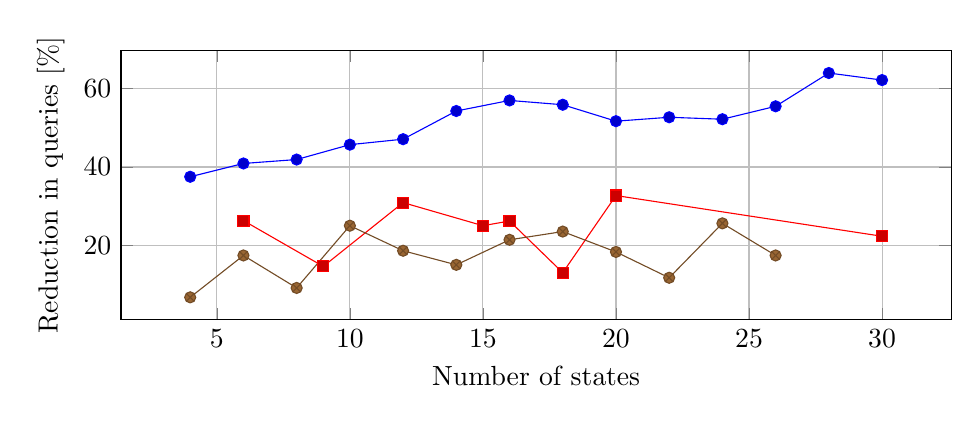
\begin{tikzpicture}
\begin{axis}[
    width=\linewidth,
    height=5cm,
    xlabel={Number of states},
    ylabel={Reduction in queries [\%]},
    legend to name=sharedlegend,
    legend columns=3,
    grid=both
]

% === Cancellation ===
\addplot coordinates {
    (4, 37.5)
    (6, 40.9)
    (8, 41.9)
    (10, 45.7)
    (12, 47.1)
    (14, 54.3)
    (16, 57.0)
    (18, 55.9)
    (20, 51.7)
    (22, 52.7)
    (24, 52.2)
    (26, 55.5)
    (28, 64.0)
    (30, 62.2)
};
\addlegendentry{Cancellation}

% === Commutativity ===
\addplot coordinates {
    (6, 26.3)
    (9, 14.6)
    (12, 30.9)
    (15, 25.0)
    (16, 26.2)
    (18, 13.0)
    (20, 32.7)
    (30, 22.3)
};
\addlegendentry{Commutativity}

% === Idempotency ===
\addplot coordinates {
    (4, 6.7)
    (6, 17.4)
    (8, 9.1)
    (10, 25.0)
    (12, 18.6)
    (14, 15.0)
    (16, 21.4)
    (18, 23.5)
    (20, 18.3)
    (22, 11.7)
    (24, 25.6)
    (26, 17.4)
};
\addlegendentry{Idempotency}

\end{axis}
\end{tikzpicture}
\caption{Reduction in the number of queries}
\end{subfigure}
\hfill
\begin{subfigure}{0.48\linewidth}
\centering
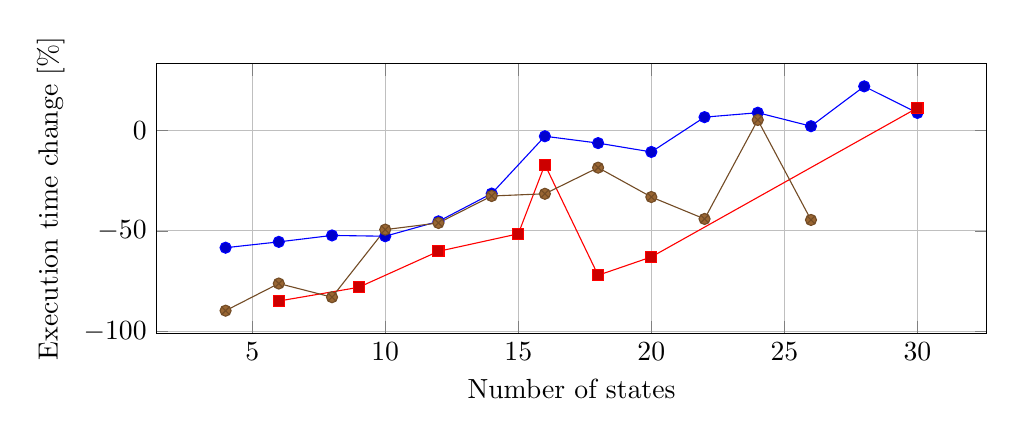
\begin{tikzpicture}
\begin{axis}[
    width=\linewidth,
    height=5cm,
    xlabel={Number of states},
    ylabel={Execution time change [\%]},
    grid=both
]

% === Cancellation ===
\addplot coordinates {
    (4, -58.4)
    (6, -55.5)
    (8, -52.3)
    (10, -52.7)
    (12, -45.3)
    (14, -31.5)
    (16, -3.0)
    (18, -6.4)
    (20, -10.8)
    (22, 6.5)
    (24, 8.7)
    (26, 2.0)
    (28, 21.8)
    (30, 8.6)
};

% === Commutativity ===
\addplot coordinates {
    (6, -84.9)
    (9, -78.1)
    (12, -60.2)
    (15, -51.5)
    (16, -17.1)
    (18, -72.1)
    (20, -63.0)
    (30, 11.1)
};

% === Idempotency ===
\addplot coordinates {
    (4, -89.7)
    (6, -76.2)
    (8, -83.0)
    (10, -49.4)
    (12, -46.1)
    (14, -32.7)
    (16, -31.6)
    (18, -18.6)
    (20, -33.2)
    (22, -44.1)
    (24, 5.1)
    (26, -44.6)
};

\end{axis}
\end{tikzpicture}
\caption{Relative change in execution time}
\end{subfigure}

\vspace{2mm}
\ref{sharedlegend}

\caption{Impact of SRS on the number of equivalence queries and execution time across different SRS rule types}

\end{figure}

\FloatBarrier

\Paragraph{The probabilistic setting}
%In this section, we evaluate two aspects: the impact of SRS on reliability and the reduction in processing time.
Since the \SRS enables equivalence testing to be performed in two stages, 
we compare the algorithm with advice against the baseline, using two configurations for the latter: 
$10^5$ and $2 \cdot 10^5$ random words.
The second configuration checks whether the improvements observed with advice are genuinely due to the \SRS, 
rather than a result of evaluating a larger number of random words.
The experimental setup consists of $10^4$ randomly generated automata with $10$--$25$ states.
%The input alphabet was generated individually for each automaton, with slight variations depending on the considered property.
%In particular, the number of symbols of each type ranged from $2$ to $5$, while the number of stack symbols ranged from $2$ to $16$.
The number of well-matched words used for substitutions was limited to $200$.

\begin{table}[H]
\centering
\begin{tabular}{cc|ccc}
\hline
SRS rule & Metric
& $10^5$ random words
& $2\cdot10^5$ random words
& $10^5$ with SRS \\
\hline
\multirow{2}{*}{Cancellation}
& Success ratio & 30.29\% & 40.1\% & 57.19\% \\
& Avg. time [s] & 0.69 & 1.28 & 2.6 \\
\hline
\multirow{2}{*}{Commutativity}
& Success ratio & 73.93\% & 78.59\% & 74.11\% \\
& Avg. time [s] & 0.69 & 0.89 & 2.0 \\
\hline
\multirow{2}{*}{Idempotency}
& Success ratio & 91.0\% & 93.24\% & 91.69\% \\
& Avg. time [s] & 0.38 & 0.78 & 0.92 \\
\hline
\end{tabular}
\caption{Comparison of success ratio and average execution time for different SRS rule types}
\end{table}

\Paragraph{Summary}
Our results show a reduction of approximately $20\%$ in the equivalence queries for commutativity and idempotency,
and around $50\%$ for cancellation rules. 
While time measurements indicate that the \SRS generally increases execution time, it reduces it for the largest instances, suggesting the benefit grows with automaton size.
Based on prior experiments for \DFA~\cite{ecai25}, we expected significant gains for commutativity; however, the results differ.
We suspect the generated \DVPA consistent with commutativity were too simple for the advice to significantly impact performance.
Reliability results did not show a dramatic improvement, but the \SRS did improve the success ratio.
The overhead mainly stems from the auxiliary heuristic for selecting well-matched words. 
While this cost is negligible compared to an exact check, it is noticeable in the probabilistic setting. 
However, if word evaluation becomes more expensive (e.g., using an LLM to evaluate words instead of \DVPA), this overhead vanishes, suggesting \SRS is a valuable feature for heuristic approaches.
 
